\section{Kuala Lumpur}

17 mai 2008

\begin{multicols}{2}

On entamme la Malaisie...

Eh oui, nous voici donc en Malaisie, toujours dans le détroit de Malacca séparant l'Indonesie et la Malaisie. Nous avons décidé de faire une escale avant Langkawi, notre dernier arrêt avant d'entrer en Thaïlande. Ce sera Port Dickson, proche de Kuala Lumpur (KL pour les intimes). Nous arrivons à Port Dickson et là, surprise, on nous annonce qu'il y a un gros festival qui va se dérouler pendant les trois jours où nous sommes là, le Freedom Festival. C'est une sorte d'eurockéennes mais avec que de la musique techno-boum-boum, ils en raffolent ici...

Oui, mais bon, nous c'est pas notre truc... On préfère aller visiter Kuala Lumpur, on se renseigne sur comment y aller : ce sera 1/4h de bus, changement, 1h de bus, puis 1h de train. On nous a dit de descendre à KLCC, c'est là qu'il y a des trucs à voir. En fait il s'agit d'espèces de galeries Lafayette de luxe : Gucci, Armani, Chanel... Ce qui nous fait croire que KLCC veux dire Kuala Lumpur Chopping Center, si vous avez une autre proposition je suis preneur. Nous pas contrariants, on y va, on sort de la station, on lève les yeux et regardez ce que l'on voit :

%\hspace*{-0.65cm}
%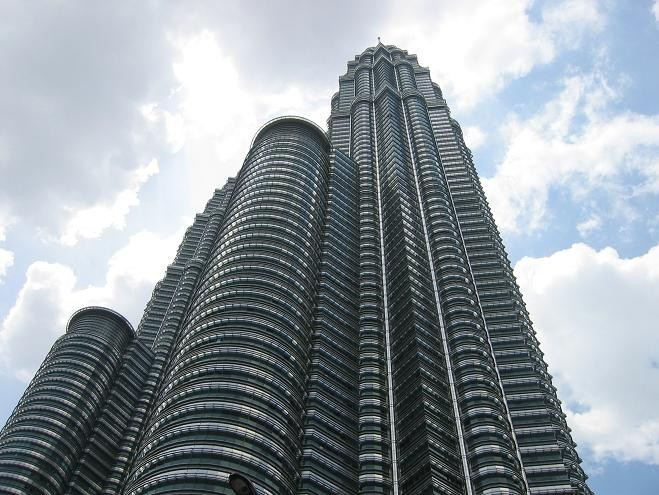
\includegraphics[width=4.8cm]{articles/Kuala-lumpur/1210432312E0e6.jpg}
%Tours Petronas.

Vous reconnaissez ? ce sont les tours jumelles très connues de Kuala Lumpur, elles répondent au petit nom de tours Petronas et sont les tours jumelles encore debout les plus hautes du monde, il paraîtrait qu'il y a une banque au sommet, et c'est ici qu'a été tourné la fin du film Haute Voltige avec Sean Connery.

On continue et qu'est-ce que je vois... un bob AE qui se promène... il paraît qu'il fait le tour du monde (pour ceux qui ne voient pas de quoi je parle, rendez vous à la fin de l'article).

%\hspace*{-0.65cm}
%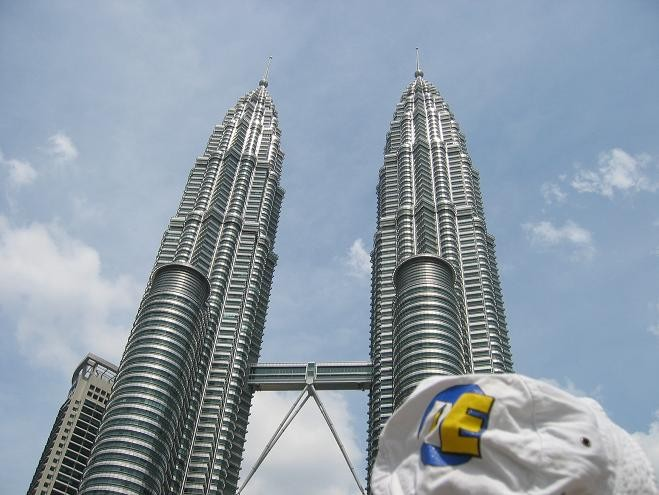
\includegraphics[width=4.8cm]{articles/Kuala-lumpur/1210432316GlgU.jpg}
%Tours Petronas again.

Allez c'est décidé on marche un peu, on mange un bout, et au detour d'une rue...

%\hspace*{-0.65cm}
%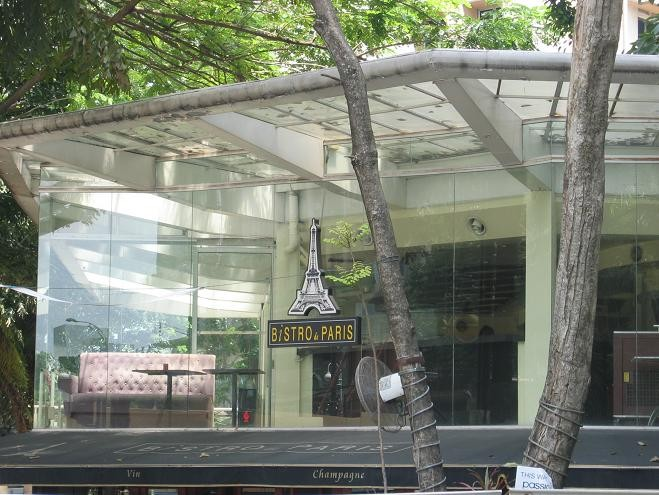
\includegraphics[width=4.8cm]{articles/Kuala-lumpur/1211015560vRGE.jpg}
%Un peu de chauvinisme.

Y a pas à dire la tour Eiffel et Zidane, restent les deux éléments connus partout dans le monde quand on parle de la France.

Bon c'est pas tout ça mais nous on lève encore les yeux au ciel et on voit encore des choses sympa, en particulier cette tour, la 4ème la plus haute du monde avec ses 421 mètres de haut.

%\hspace*{-0.65cm}
%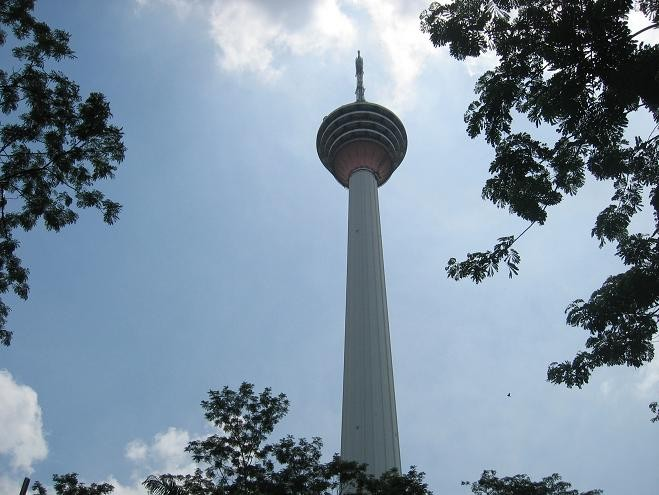
\includegraphics[width=4.8cm]{articles/Kuala-lumpur/1211014906Nl6S.jpg}
%Tour qui s'appelle je sais plus comment.

Qu'est-ce qu'on doit avoir une belle vue de là haut... allez hop on y va...

%\hspace*{-0.65cm}
%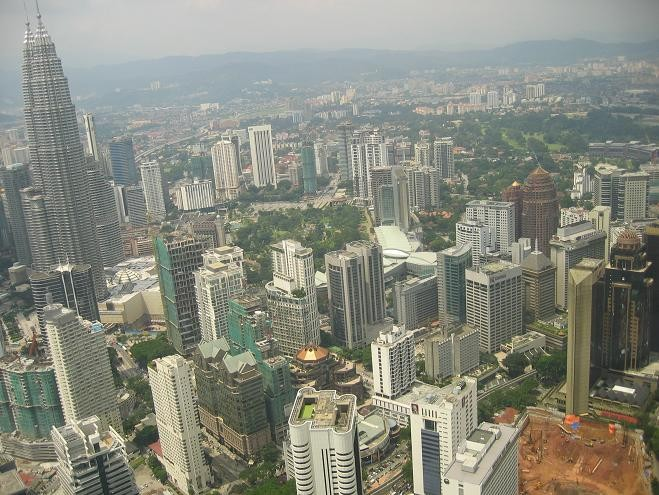
\includegraphics[width=4.8cm]{articles/Kuala-lumpur/1211014913RrBL.jpg}
%Vue d'en haut de la tour (qui tourne...)

Moi qui adore voir les choses de loin, et du plus haut possible, j'étais servi. Kuala Lumpur sur 360 degrés.

Retour sur le plancher des singes, en dehors de ses gratte-ciel KL redevient une ville ressemblant à beaucoup de capitales, si ce n'est que tout est nickel, presque comme à Singapour. Mais allez savoir pourquoi, à KL je me sentais bien, loin de l'impression que j'ai eu à Singapour.

Je vous laisse sur deux photos de la ville en elle même.

%\hspace*{-0.65cm}
%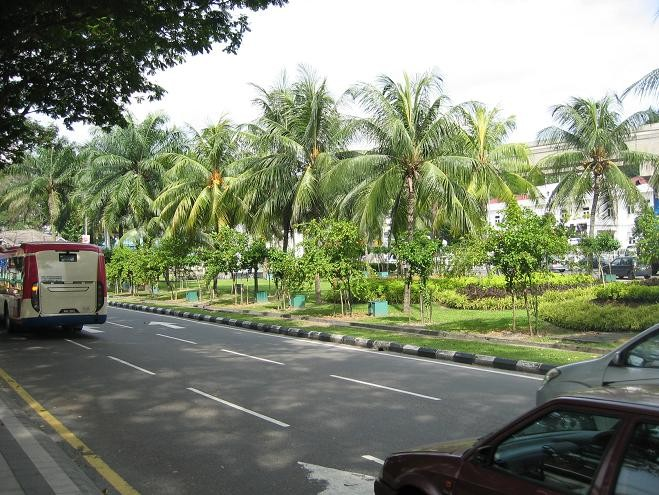
\includegraphics[width=4.8cm]{articles/Kuala-lumpur/1211016874hbIL.jpg}
%Ben... la rue quoi.

%\hspace*{-0.65cm}
%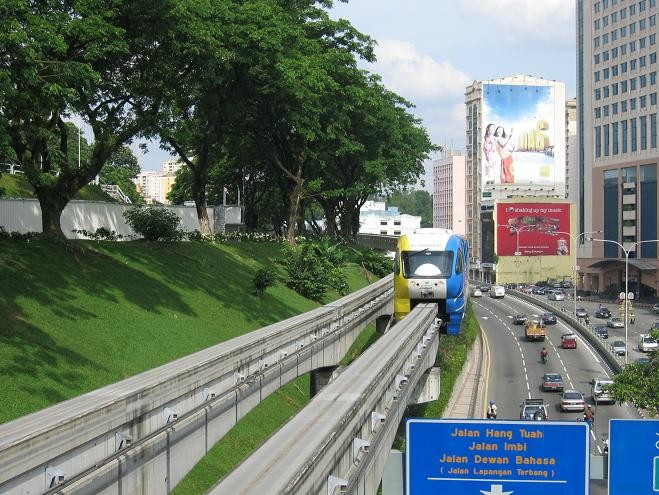
\includegraphics[width=4.8cm]{articles/Kuala-lumpur/1211017229ryCi.jpg}
%Monorail aérien.

\end{multicols}

 * Le bob autour du monde, kesako ? A l'UTBM il y a eu un message de passé incitant toutes les personnes voyageant autour du monde à emporter un bob AE (Association des Etudiants) et à le prendre en photo devant les grands endroits connus où l'on pourrait aller.

\bigskip
\textbf{\textsc{Commentaires}}

\medskip
Titou a écrit le 18 mai 2008 :
\begin{displayquote}
Je n'ai qu'une chose à dire : petit enfoiré ! C'est franchement magnifique ! Tu m'étonnes que tu te sentes bien là-bas. Merci de prendre quelques instants pour nous en faire profiter, ça fait du bien de voyager un peu par ces temps de gros taff. Continue de t'éclater et à plus ! Biz mon pote !
Ps : ton truc anti-spam ça claque! Après faut gérer les additions\dots t'as pa pensé à ça toi! heureusement on a pu m'aider pour répondre :p
\end{displayquote}

\medskip
Peggy a écrit le 18 mai 2008 :
\begin{displayquote}
Pareil que "titou" je suis en panique là, je me concentre fort pour ne pas oublier la réponse au fameux calcul anti-spam (aujourd'hui: 8+2) et du coup je conclue très vite en te faisant des biz.
SEE YOU.
\end{displayquote}

\medskip
Etienne a écrit le 19 mai 2008 :
\begin{displayquote}
Ah oui évidement les pré-requis sont peut être un peu élevés pour certains, mais en s'y mettant à plusieurs pour repondre je pense que c'est faisable.
Merci à vous deux qui prenez toujours le temps de laisser un message, les autres vous savez quoi faire, et à tous les "occasionnels", qui ont peut être étés refroidis par le spam, ça y est c'est fini, vous pouvez revenir !
Je vous promet encore des superbes photos pour venir compléter l'article sur Langkawi, cette île est vraiment top!!!
\end{displayquote}

\medskip
Gege (rien) a écrit le 19 mai 2008 :
\begin{displayquote}
Alors pour ceux à qui le petit calcul fait tellement peur : Menu démarrer --> Programmes --> accesoires --> calculatrice :)
Des tours aussi hautes, ça me fout tout le temps le vertige : j'imagine même pas les jours de grands vents, comment la tour doit bouger, ça doit foutre la g****
\end{displayquote}

\medskip
Zan a écrit le 19 mai 2008 :
\begin{displayquote}
Et dire que j'étais dans cette ville il y a un peu plus d'un an et que j'ai rien vu de tout ça!!! C'est super beau, grand\dots
Enfin bon c'est ça d'avoir juste 2 heures d'escale à Kuala Lumpur en faisant Paris-Sydney, je suis pas sorti de l'aéroport\dots Mais bon ce sera pour une prochaine fois :D
Enjoy, c'est vraiment magnifique tout ça!
\end{displayquote}

\vfill

